\documentclass[11pt,a4paper]{report}
\usepackage{graphicx}
\usepackage{titlepic}
\usepackage{helvet}
\renewcommand{\familydefault}{\sfdefault}
\setlength{\parskip}{1em}
\usepackage{listings}
\usepackage{color}

\definecolor{dkgreen}{rgb}{0,0.6,0}
\definecolor{gray}{rgb}{0.5,0.5,0.5}
\definecolor{mauve}{rgb}{0.58,0,0.82}

\lstset{frame=tb,
  aboveskip=3mm,
  belowskip=3mm,
  showstringspaces=false,
  columns=flexible,
  basicstyle={\small\ttfamily},
  numbers=none,
  numberstyle=\tiny\color{gray},
  keywordstyle=\color{blue},
  commentstyle=\color{dkgreen},
  stringstyle=\color{mauve},
  breaklines=true,
  breakatwhitespace=true,
  tabsize=3
}

\title{
\includegraphics[scale=1.5]{twt}\\~\\~\\ \LARGE{\textbf{TWT Programming
Language}}\\~\\ \large{(Talagang Walang Tulog)}\\~\\ \large{Language Manual}}
\date{~\\ December 2015}
\author{Jahziel Rae Arceo\\ Gabriel Kelly Navarro\\ Mikaela Jun Lenon\\ Maria
Rosario Gueco\\ Marbille Juntado\\~\\~\\ CS 150 HTWX}

\begin{document}

\maketitle

\section*{Text editor}

\begin{center}
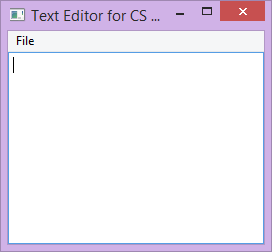
\includegraphics[scale=0.75]{TextEditor001}
\end{center}

The file editor for the language automatically formats the saved file to a .twt
file extension. This text editor can be used for editing the code, and making it
sure it goes through TWT language specifications.

\section*{Compiling the code}

The TWT programming language has its compiler (converter) named "try".\par

\noindent The TWT code can be run by this command-line input:

\begin{lstlisting}
try <filename>
\end{lstlisting}

Note that filename doesn't have ".twt" on its argument. The compiler makes sure
that it is only processing TWT source codes.

Error codes are seen on the console if there are any problems about the code.

\section*{Running the code}

After compilation, the program will commence. After program run, it ill
automatically close in 10 seconds.

\end{document}
